\documentclass[a4paper, 12pt]{article}

\usepackage{cmap}
\usepackage{mathtext} 
\usepackage[T2A]{fontenc}
\usepackage[utf8]{inputenc}
\usepackage[english,russian]{babel}

\usepackage{amsfonts,amssymb,amsthm,mathtools}
\usepackage{amsmath}
\usepackage{icomma} 

\usepackage{graphicx} 
\graphicspath{{Picturies/}}
\usepackage{wrapfig}

\usepackage{array,tabularx,tabulary,booktabs}
\usepackage{longtable}
\usepackage{multirow}

\usepackage{caption}
\usepackage{subcaption}
\captionsetup{labelsep=period}

\renewcommand{\phi}{\varphi}
\newcommand{\eps}{\varepsilon}
\renewcommand{\AA}{\ensuremath{\mathring{A}}}
\newcommand{\parag}[1]{\paragraph*{#1:}}

\newcounter{Points}
\setcounter{Points}{1}
\newcommand{\point}{\arabic{Points}. \addtocounter{Points}{1}}

\author{Вязовцев Андрей, Б01-005}
\date{20.05.22}
\title{Лабораторная работа 4.1.2. Моделирование оптических приборов и определение их увеличения.}

\begin {document}

\maketitle

\parag {Цель работы} моделирование оптических приборов и определение их увеличения.

\parag {В работе используются} оптическая скамья, набор линз, экран, осветитель со шкалой, зрительная труба, диафрагма, линейка.

\parag {Теоретическая справка} ~\\

Формула для расчета фокусного расстояния рассеивающей линзы с помощью зрительной трубы
\begin{equation}
	\label{eq1}
	f~=~l~-~a_0
\end{equation}

где $l$~---~расстояние между линзами, $a_0$~---~расстояние между собирающей (вспомогательной) линзы.

Формула для расчета увеличения:
\begin{equation}
	\label{eq2}
	N~=~\dfrac{\alpha'}{\alpha}~=~\dfrac{f_1}{f_2}~=~\dfrac{h_2}{h_1}
\end{equation}

где $f_1,~f_2$~---~фокусные расстояние соответствующих линз (зависит от установки), $h_1$~---~размер изображения одного миллиметра шкалы осветителя в делениях окулярной шкалы зрительной трубы, $h_2$~---~размер изображения миллиметрового деления шкалы осветителя в делениях окулярной шкалы трубы (после прохождения оптического прибора).

Необходимый интервал $\Delta$(для микроскопа):
\begin{equation}
	\label{eq3}
	N_M~=~N_1 \cdot N_2~=~\dfrac{\Delta}{f_1} \dfrac{L}{f_2} 
\end{equation}

где $f_1,~f_2$~---~фокусные расстояния соответствующих линз, $L~=~25$ см~---~расстояние наилучшего зрения, $N_M$~---~увеличение микроскопа.

Длина тубуса микроскопа:
\begin{equation}
	\label{eq4}
	l_{12}~=~\Delta + f_1 + f_2
\end{equation}

Увеличение микроскопа можно найти таким образом:
\begin{equation}
	\label{eq5}
	N_M~=~\dfrac{h_2}{h_1} \dfrac{L}{f}
\end{equation}

\parag {Ход работы} ~\\

\point Определим типы линз и их фокусное расстояние на глаз. После чего центрируем систему.

Линзы $1, 2, 3, 4$~---~собирающие, линза $5$~---~рассеивающая. 

\begin{table}[!h]
\centering
\begin{tabular}{|c|c|c|c|c|} \hline
	Номер линзы & 1 & 2 & 3 & 4 \\ \hline
	f, см & $10 \pm 0.1$ & $20 \pm 0.1$ & $2 \pm 0.1$ & $30 \pm 0.1$ \\ \hline
\end{tabular}
\end{table}

\point Теперь найдём фокусные расстояния тонких линз с помощью зрительной трубы. Для этого настроим трубу на бесконечность. Установим линзу на расстоянии от предмета примерно равном фокусному. Разместим трубу на небольшом расстоянии от линзы. Передвигая линзу вдоль скамьи, получим в окуляре трубы изображение, при этом расстояние между предметом и серединой тонкой линзы равно фокусному.

\begin{figure}[!h]
	\centering
	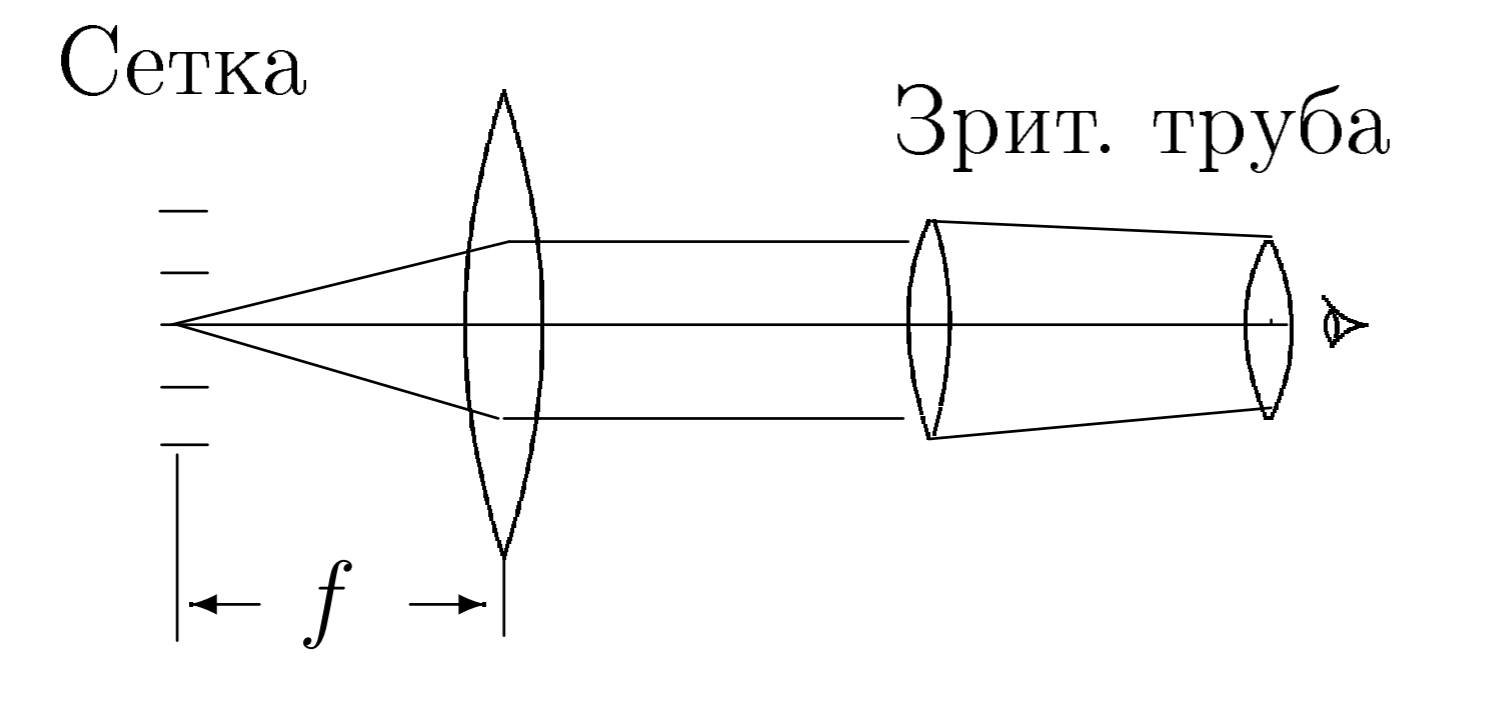
\includegraphics[scale = 0.3]{412-1.png}
	\caption{Определение фокусного расстояние собирающей линзы}
	\label{pic1}
\end{figure}

Запишем измеренные фокусные расстояния для собирающих линз\\
	
\begin{table}[!h]
\centering
\begin{tabular}{|c|c|c|c|c|c|} \hline
	Номер линзы & 1 & 2 & 3 & 4 \\ \hline
	f, см & $7.5 \pm 0.5$ & $11.5 \pm 0.5$ & $2.0 \pm 0.5$ & $30.0 \pm 0.5$ \\ \hline
\end{tabular}
\end{table}

\point Для определения фокусного расстояния рассеивающйе линзы сначала получим увеличенное изображение сетки с помощью одной короткофокусной лины ($F_1 = 7.5$ см). Измерим расстояние между линзой и экраном: $a_0 = 19.0 \pm 0.5$ см. Разместим сразу за экраном трубу, уберем экран и, перемещая рассеивающую линзу, найдем в окуляре трубы изображение сетки. Измерим расстояние между линзами $l = 32.0 \pm 0.5$ см. Таким образом получаем $F_5 = -13.0 \pm 0.5$ см.

\begin{figure}[!h]
	\centering
	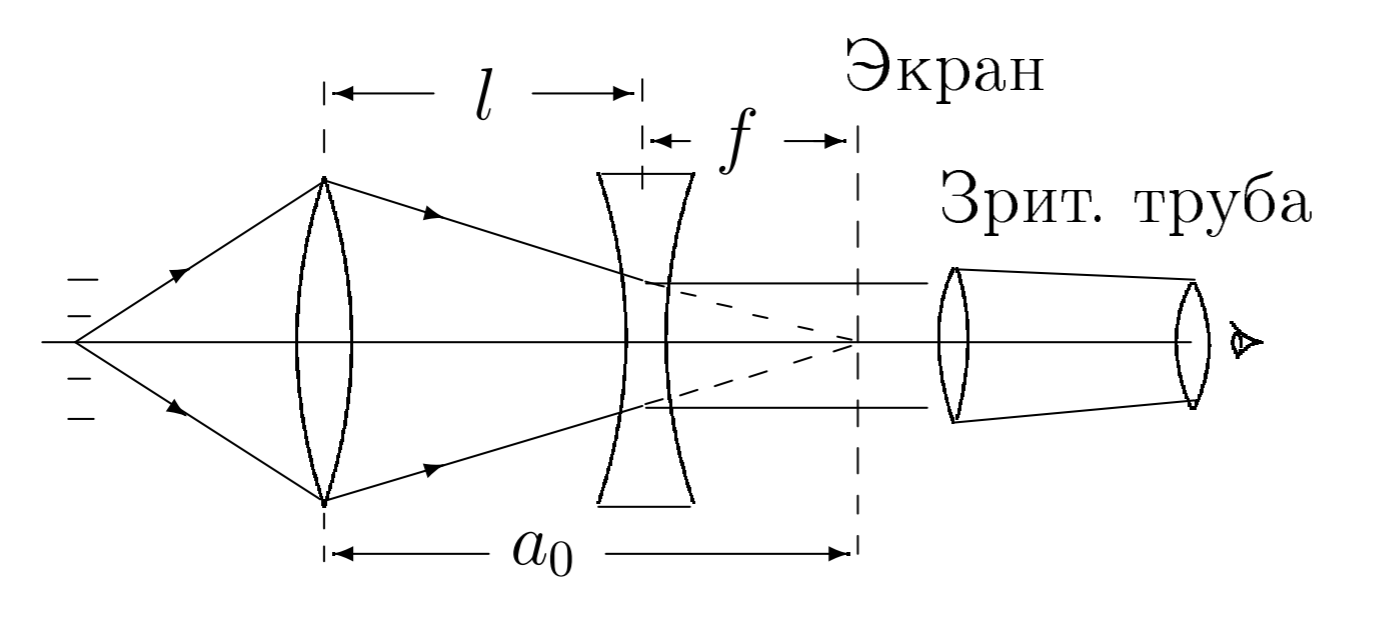
\includegraphics[scale = 0.4]{412-2.png}
	\caption{Определение фокусного расстояние рассеивающей линзы}
	\label{pic2}
\end{figure}

\point Телескоп Кеплера. Выберем две собирающие линзы (под номерами 2 и 1) для создания модели трубы Кеплера. В качестве коллиматора используем линзу 3.

\begin{figure}[!h]
	\centering
	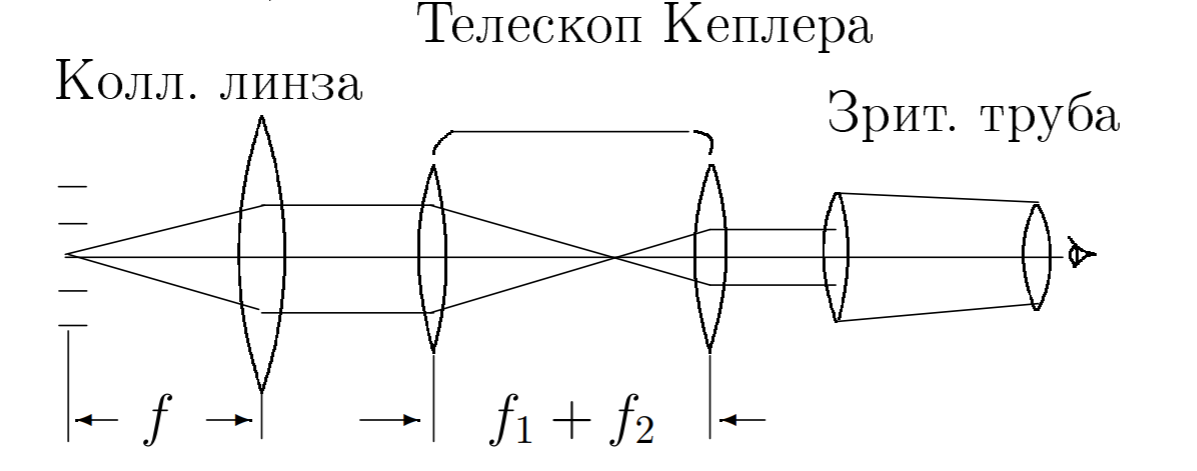
\includegraphics[scale = 0.5]{412-3.png}
	\caption{Модель телескопа Кеплера}
	\label{pic3}
\end{figure}

Соберем модель телескопа, используя расстояния, которые расчитаны на основе фокусов (см. \ref{pic3}).1  Слегка перемещая окуляр модели, получим изображение миллиметровой сетки в окуляре трубы.

\point Измерим расстояние между объективом и окуляром: $L = 30.0 \pm 0.5$ см. Примерно совпадает с суммой фокусных расстояний ($30$ см).

\point Посмотрим на изображение в телескопе и без него. С ним: $h_1 = 9 \pm 1$ дел., без: $h_2 = 6 \pm 1$ дел.

\begin{equation*}
	N_Т = \frac{f_1}{f_2} = 1.5 \pm 0.1
\end{equation*}

\begin{equation*}
	N_T = \frac{h_1}{h_2} = 1.5 \pm 0.2
\end{equation*}

\point Труба Галилея. Труба Галилея имеет такую же схему, как и телескоп Кеплера, только вместо собирающей окулярной линзы поставить рассеивающую на расстоянии от объектива, равном разности фокусов объектива и окуляра. Далее все измерения аналогичны телескопу Кеплера. $h_2 = 22$ дел.

\begin{equation*}
	N_Т = \frac{f_1}{f_2} = 2.3 \pm 0.1
\end{equation*}

\begin{equation*}
	N_T = \frac{h_1}{h_2} = 3.7 \pm 0.2
\end{equation*}

\point Модель микроскопа. К сожалению, этот пункт не был сделан.

% \begin{table}[!h]
% 	\centering
% \begin{tabular}{|c|c|c|c|c|c|} \hline
% 	№ решетки & 1 & 2 & 3 & 4 & 5 \\ \hline
% 	Расстояние, мм & 31.3 & 21.0 & 10.5 & 5.2 & 4.3 \\ \hline
% \end{tabular}
% \end{table}

% \begin{figure}[!h]
% 	\centering
% 	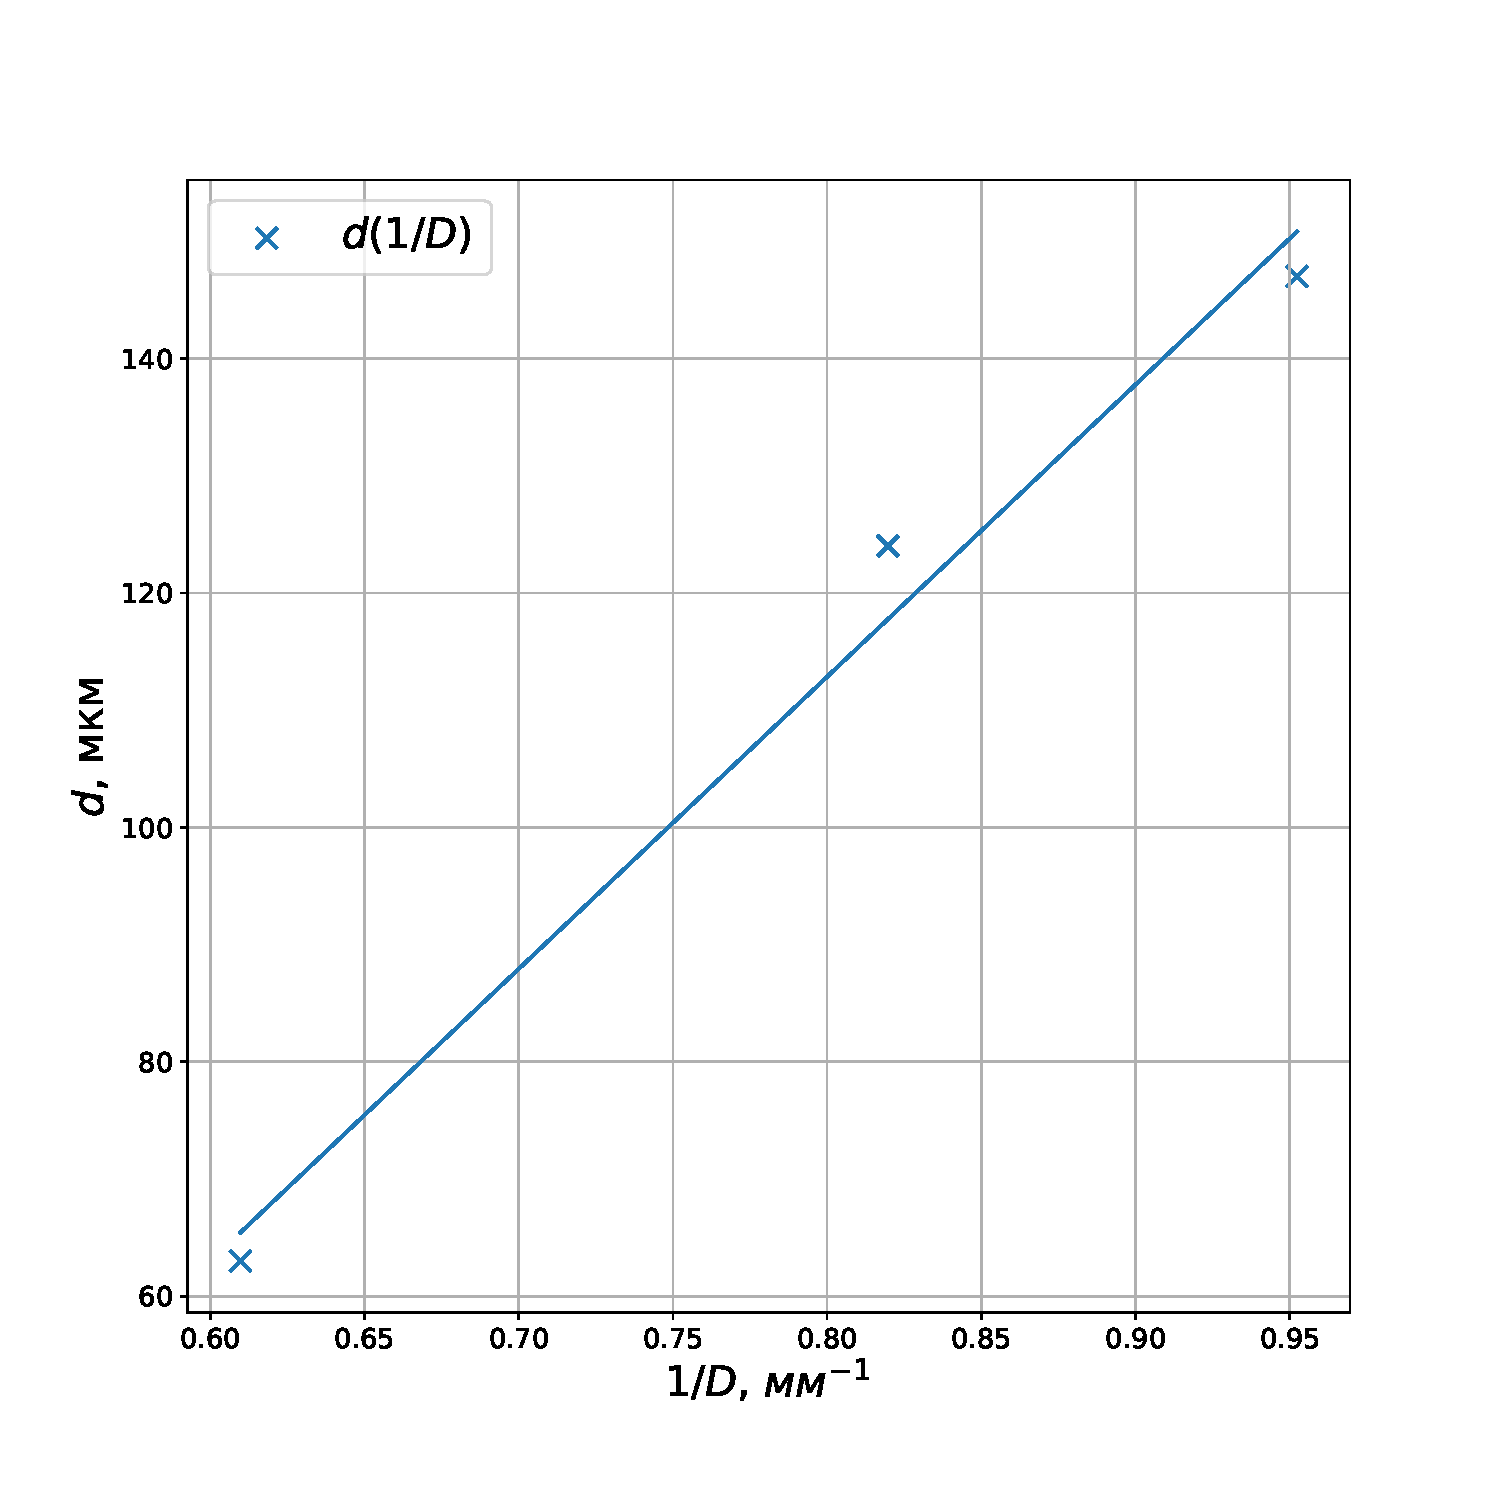
\includegraphics[scale = 0.4]{graph1}
% 	\caption{График зависимости $d = f \left( 1 / D \right)$}
% 	\label{graph1}
% \end{figure}

\end {document}
